\documentclass[a4paper,twoside,12pt,nochapterprefix]{scrbook}


\usepackage{amsmath,amssymb,amsthm}
\usepackage[footnotesize,sl,SL,hang,tight]{subfigure}  % helpful package for aligning figures next to each other
\usepackage{longtable} % tables over several pages
\usepackage[font={small,sl},hang,labelfont=bf]{caption} % configure captions
\usepackage{booktabs} % publication quality tables for LaTeX
%\usepackage{showkeys} % shows the labels above the references for easier development

\ifpdfoutput{%
	\usepackage[pdftex]{graphicx}
	\usepackage[]{pdfpages} %for including full pdf pages
}{%
	\usepackage{graphicx}
}
\usepackage{epstopdf}
\epstopdfsetup{update} % only regenerate pdf files when eps file is newer

\usepackage{rotating} % rotate figures

\usepackage[headinclude]{scrpage2}
\usepackage{multirow}


% Font packages:
\usepackage{times}
\usepackage{helvet}   % sets sans serif font
\usepackage[T1]{fontenc}
\usepackage{blindtext}
\usepackage{amsmath}
\usepackage[linesnumbered,ruled]{algorithm2e}

\usepackage{tikz}
\usepackage{blkarray}
\usepackage{amsmath}
\usepackage{tikz,forest}
\usetikzlibrary{arrows.meta}
\usetikzlibrary{trees}
\usepackage{booktabs}
\usepackage{multirow}
\usepackage{siunitx}





%PDF hyperref config
\ifpdfoutput{%
	\usepackage[pdftex,
		a4paper,
		bookmarks,
		bookmarksopen=true,
		bookmarksnumbered=true,
		pdfauthor={Jacqueline Staub},       % FILL THIS IN PROPERLY
		pdftitle={Sound Analysis on low Quality Microphones: An Approach to a game-based Android Application},   % FILL THIS IN PRPERLY
		colorlinks,
		linkcolor=black,
		citecolor=black,
		filecolor=black,
		urlcolor=black,
		anchorcolor=black,
		menucolor=black,
		breaklinks=true,
		pageanchor=true,
		plainpages=false,
		pdfpagelabels=true]{hyperref}
}{}

\ifpdfoutput{%
	\pdfcompresslevel=9
	\pdfoutput=1
	\DeclareGraphicsExtensions{.pdf,.png}
}{}

%\bibliographystyle{abbrv-fr}
\bibliographystyle{acmsiggraph}



% A4
%
\topmargin -0.5in
\textheight 9.3in
\textwidth 6.3in
\oddsidemargin 0.18in
\evensidemargin -0.22in
\parskip 0.1in
\parindent 0in

\renewcommand{\arraystretch}{1.5}
\renewcommand{\baselinestretch}{1}

% !TEX root = ../thesis.tex

% TO DO search symbol
\newcommand{\TODO}{\mbox{\large\bf TO DO}}
\newcommand{\REFR}{\mbox{\large\bf REFR}}

%  Terminates current page and paragraph, makes sure next page starts on
%  an odd-number, and generates a completely blank page, without page markers,
%  if necessary.
\newcommand{\clearemptydoublepage}{\newpage{\pagestyle{empty}\cleardoublepage}}


% !TEX root = ../thesis.tex

% Stripped from acm siggraph bst and cls
\makeatletter

% no labels in bibliography.
\def\@biblabel#1{}

\newlength{\bibhang}
\setlength{\bibhang}{1em}

% Change in-bibliography biberence style
\def\thebibliography#1{%
  \section*{%
    \bibname\@mkboth{\sl\uppercase{\bibname}}{\sl\uppercase{\bibname}}}
  \list{\relax}{\setlength{\labelsep}{0em}
                \setlength{\itemindent}{-\bibhang}
                \setlength{\leftmargin}{\bibhang}}
  \def\newblock{\hskip .11em plus .33em minus .07em}
  \sloppy\clubpenalty4000\widowpenalty4000
  \sfcode`\.=1000\relax}

% Not sure what this does...
%\def\@citex[#1]#2{\if@filesw\immediate\write\@auxout{\string\citation{#2}}\fi
%  \def\@citea{}\@cite{\@for\@citeb:=#2\do
%    {\@citea\def\@citea{; }\@ifundefined
%      {b@\@citeb}{{\bf ?}\@warning
%      {Citation '\@citeb' on page \thepage \space undefined}}%
%{\csname b@\@citeb\endcsname}}}{#1}}

% Change in-document citation styles
\let\@internalcite\cite
\def\cite{\def\citename##1{##1}\@internalcite}
\def\shortcite{\def\citename##1{}\@internalcite}
%\def\numcite{\def\citeyear{}\@internalcite}

\makeatother


\begin{document}

%% Define leading chapter pages
%
% !TEX root = ../thesis.tex

\addtokomafont{chapter}{\setlength{\parskip}{190pt}}   % SEVERE HACK to keep spacing to chapter art work
%\addtokomafont{chapter}{\rmfamily}        % remove this if you prefer sans-serif section titles
%\addtokomafont{section}{\rmfamily}        % remove this if you prefer sans-serif section titles
%\addtokomafont{subsection}{\rmfamily}     % remove this if you prefer sans-serif section titles
%\addtokomafont{subsubsection}{\rmfamily}  % remove this if you prefer sans-serif section titles
%\addtokomafont{paragraph}{\rmfamily}      % replace by \sffamily if you prefer sans-serif para titles
\addtokomafont{paragraph}{\sffamily}

\def\mychpstyleintl{%
{\noindent\setlength{\tabcolsep}{0pt}\setlength{\arrayrulewidth}{2pt}%
\begin{tabular}{c}
\\[100pt]
\begin{tabular}{lr}
\begin{tabular}{p{0.6\linewidth}}
\\
\end{tabular}
&
\begin{tabular}{p{0.4\linewidth}}
\rightline{{%
\sffamily%
\fontseries{bx}%
\fontshape{n}%
\fontsize{100}{120}%choose baselineskip to be 1.2 times font size
\selectfont
\thechapter}}
\end{tabular}
\end{tabular}\\[300pt]
\end{tabular}
}}

\newpagestyle{mychapterpagestyle}{{\protect\mychpstyleintl}{\protect\mychpstyleintl}}{}
\newpagestyle{myappendixpagestyle}{{\protect\mychpstyleintl}{\protect\mychpstyleintl}}{}
%%

%% macros e.g.
\newcommand{\mfytext}[0]{my fancy text}

%refs
\newcommand{\chpref}[1]{Chapter \ref{#1}}
\newcommand{\secref}[1]{Section \ref{#1}}
%\newcommand{\equref}[1]{Equation \ref{#1}} %better use builtin \eqref{}
\newcommand{\figref}[1]{Figure \ref{#1}}
\newcommand{\tabref}[1]{Table \ref{#1}}
\newcommand{\apxref}[1]{Appendix \ref{#1}}
%%

%% Replace this by your own design of a title page
%
%\title{Sound analysis on smartphones}
%\author{Jacqueline Staub}
%\date{March 2014}
%\maketitle
%\clearemptydoublepage
% --- selfmade version ----
\begin{titlepage}
	\topmargin 1.0cm
	\oddsidemargin 0.0cm
	\evensidemargin 0.0cm
	%\textwidth 6.5in
	\centering
	\Huge
	\vspace{3.0cm}
	\textbf{\textsf{Fast Polyhedra Analysis with deep Q-networks}} \\[2.0cm]
	\vspace{3cm}
	\sffamily
	\Large
	Jakub Kotal
	\\[0.8cm]
	\large
	Bachelor Thesis
	\\
	Novemeber 2018
	\\[1.3cm]
	\emph{Supervisor:}\\
	%Dr.\ My Supervisor\\ 					% The name of the thesis supervisor
	Phd.\ Singh Gagandeep, 		% The supervising professor\\
	Prof.\ Dr.\ Martin Vechev		% The supervising professor
	\vfill
	\begin{center}
		\includegraphics*[height=0.8cm]{figures/eth_logo_kurz_pos.eps} \hfill 
	\end{center}
	
	\vspace{3.4cm}
\end{titlepage}
\clearemptydoublepage
%%

\pagenumbering{roman}
\setcounter{page}{1}

% !TEX root = ../thesis.tex

%TODO finish abstract
\chapter*{Abstract}
We use deep Q-networks to increase the performance of numerical analysis whilst maintaining a sufficient precision. In this work, we build upon an existing framework that uses linear basis function approximation in order to model a decision policy for leveraging precision loss for performance gain inside of polyhedra analysis. We expand this framework with the use of nonlinear deep Q-networks for the Q-function approximation. We then further optimise this method by testing new features, reward functions as well as other problem specific optimisations. We also try to increase the flexibility of the proposed algorithm. Finally, we train and test our resulting algorithm, with which we are able to achieve a considerable gain in both performance and precision.


% !TEX root = ../thesis.tex

\chapter*{Acknowledgment}

I would like to thank Prof. Dr. Otmar Hilliges for supervising this project. Thanks to him I had the opportunity to get to know many fields in computer science that were unfamiliar to me half a year ago. The last semester was a very challenging and rewarding one. His profound knowledge in many areas was very helpful to me.

Furthermore i would like to express my deep appreciation and gratitude to Christine Ryer-Bringold, my former music teacher. She supported me generously with many hours of supportive advices and conversations about education and music. 

Someone else who deserves my deep gratitude is my mother. The innumerable sacrifices she made to support me whenever she could are highly appreciated and I cannot say how thankful I am for everything she did.


%-----------------------------------------------------------------------------------------------
%include task description here:
\cleardoublepage
%\includegraphics[viewport=3cm 0cm 20cm 27.5cm]{task_description} %better use includepdf below!
%\includepdf{task_description}
\cleardoublepage
%-----------------------------------------------------------------------------------------------

%include acknowledgment here:
%% !TEX root = ../thesis.tex

\chapter*{Acknowledgment}

I would like to thank Prof. Dr. Otmar Hilliges for supervising this project. Thanks to him I had the opportunity to get to know many fields in computer science that were unfamiliar to me half a year ago. The last semester was a very challenging and rewarding one. His profound knowledge in many areas was very helpful to me.

Furthermore i would like to express my deep appreciation and gratitude to Christine Ryer-Bringold, my former music teacher. She supported me generously with many hours of supportive advices and conversations about education and music. 

Someone else who deserves my deep gratitude is my mother. The innumerable sacrifices she made to support me whenever she could are highly appreciated and I cannot say how thankful I am for everything she did.


\tableofcontents

\cleardoublepage
\phantomsection
\addcontentsline{toc}{chapter}{List of Figures}
%\listoffigures

\cleardoublepage
\phantomsection
\addcontentsline{toc}{chapter}{List of Tables}
%\listoftables
\cleardoublepage

\pagenumbering{arabic}
\renewcommand*{\chapterpagestyle}{mychapterpagestyle}
\renewcommand*{\chapterformat}{} % show chapter titles only (no numbers)
% \setchapterpreamble[o]{...}  unfortunately does not move the \chapter output downwards

% ---- MAIN PART ----


% !TEX root = ../thesis.tex

% set counter to n-1:
\setcounter{chapter}{0}

\chapter{Introduction}
\mbox{}\\
\mbox{}\\
\mbox{}\\
The number of domains controlled by computers has grown exponentially in the recent years. As the complexity of the structures surrounding us grows, the need for their automatision grows with it. And so, more and more the systems surrounding us, become controlled by computers. From simple things such as automatic doors to vastly more complex and important systems such as self-driving cars, medical software or nuclear weapons software. In some of these applications, a program bug could only be a slight nuisance, but in others its existence could have major implications. A few infamous examples of these exist where buffer overflows, rounding errors or division by zeros have caused space craft crashes or lethal radiation overdoses. As such, the importance of some of these devices demands their invulnerability and its verifiability. Unfortunately, as the complexity of these programs increases the need for complete and formal verification methods becomes critical.\\
Static analysis is a sub-branch of computer science. Its task is to analyse a program without its execution, its goal is to discover weaknesses inside of the code that could lead to vulnerabilities. As such, it should help with debugging and provide a better notion of safety about the code. Static analysis has seen a growing commercial use in the recent years mostly in safety-critical domains. Recent advances in this field use clever mathematical properties in order to increase the capabilities of such methods. Other techniques, leverage the domain of artificial intelligence to increase the fields capacities. For, until ai is capable of writing invulnerable software for us, we can at least use it verify ours.
\section{Problem Statement}
The main focus of static analysis is observing the effects that program expressions and statements have on the variables inside of the program. In order for these methods to work, a numerical abstract domain is needed that can capture the relationships between the variables. An important attribute of a domain is its expressivity, that is to say, how complex are the constraints between variables that the domain can represent. The more expressive a domain is the more complicated relationships it can represent. The most expressive domain is the polyhedra domain, representing the constraints with different polyhedra. However, its expressivity comes at a cost. It is notoriously time and space complex, having worst case exponential complexities in both. Other domains also exits that do not suffer from these problems. Unfortunately, to achieve this, they loose their expressivity. Modifications to the polyhedra domain are also possible, some of these modifications try to leverage precision loss against performance gain. However, finding the right balance between these two is not an easy task.

\section{Goals}
The goal of this thesis is to use some of the recent developments in new areas of reinforcement learning. To adapt and optimise these novel methods in order to to use them with polyhedra analysis. The goal is then to optimise these methods with some problem specific knowledge from polyhedra analysis, in order to render the analysis more efficient and outperform other methods.


\section{Structure of this Document}

\paragraph{Chapter 2}briefly introduces reinforcement learning, explaining the important concepts and its main goals. It will also describe some of the recent advances inside of the field and the achievements of these methods.

\paragraph{Chapter 3}addresses Polyhedra analysis. It will explain its usefulness inside of static analysers and how it works. It will also introduce some of the modifications made to the domain, in order to reduce some of its shortcomings.

\paragraph{Chapter 4}addresses the work done throughout this thesis. It will first address how the two previous chapters were combined and the basic algorithm was designed. It will also show the different methods tested to further optimise the algorithm.

\paragraph{Chapter 5}discussed the different experiments that were run to find the optimal combination of the different parts of the algorithm. It will also present the results of the execution of the finalised algorithm on different benchmarks.

\paragraph{Chapter 6}will be a final discussion of the work achieved throughout this thesis.

%TODO finish chapters results etc...









% !TEX root = ../thesis.tex

% set counter to n-1:
\setcounter{chapter}{1}

\chapter{Reinforcement Learning}
\mbox{}\\
\mbox{}\\
\mbox{}\\
Reinforcement Learning \cite{kaelbling1996reinforcement} is a very general problem of machine learning studied in a multitude of different fields, such as game theory, information theory or statistics. It is a very broad concept and the foundations are the following. An agent interacts with a given environment, at its disposal, it has a set of various actions. When an action is performed it receives a reward. The goal of the agent is to devise an action selection policy that should maximise the cumulative reward of the selected actions.

\begin{figure}[h]
	\begin{center}
		\includegraphics*[height=5cm]{figures/rl_broad.png}
		\caption{ Concepts of RL illustration \protect\cite{wiki:rl}}	
	\end{center}
\end{figure}

\section{Concepts}
In order to be able to solve a problem with reinforcement learning, it first has to be mapped to the following RL concepts:
\begin{itemize}
	\item A set of agent states $S$, with the initial state $s_0\in S$
	\item A set of actions $A$
	\item A function giving the reward of performing an action from  $s_t$ to $s_{t+1}$, $r(s_t,a_t,s_{t+1})\in \mathbb{R}$
\end{itemize}
During the execution of the program, the agent will first start in the initial state $s_0$. Then, at each timestep $t=0,1,...,$ the agent will pick an action $a_t \in A$, this action will then be executed, the agent will move from $s_t$ to $s_{t+1}$ and receive the corresponding reward $r(s_t,a_t,s_{t+1})$. This process will be repeated until a final state is reached. In RL, state transitions typically satisfy the Markov property. This property states that the next state $s_{t+1}$ only depends on the current state $s_t$ and on the action taken at this state $a_t$. We call the sequence of actions and states from the initial to the final state an episode. The goal of the agent is to devise an action selection policy so as to maximise the cumulative reward. The cumulative reward is measured as the sum of the rewards inside of an episode. We will demonstrate this reward with the following example.
\paragraph{Example 2.1}\mbox{}\\
Let's assume we have an episode with two time-steps and an action set with only two possible actions. In the following tree, we can see the different actions we can take at each state and their respective reward.\\
\begin{figure}[h]
\tikzstyle{level 1}=[level distance=3.5cm, sibling distance=3.5cm]
\tikzstyle{level 2}=[level distance=3.5cm, sibling distance=2cm]

% Define styles for bags and leafs
\tikzstyle{bag} = [text width=4em, text centered]
\tikzstyle{end} = [circle, minimum width=3pt,fill, inner sep=0pt]

\begin{center}
	
\begin{tikzpicture}[grow=right, sloped]
\node[bag] {$s_0$}
    child {
        node[bag] {$s_1$}        
            child {
                node[end, label=right:
                    {$s_3,-5 + 10 = 5$}] {}
                edge from parent
                node[above] {$a_1$}
                node[below]  {$10$}
            }
            child {
                node[end, label=right:
                    {$s_4,-5 + 30 = 25$}] {}
                edge from parent
                node[above] {$a_0$}
                node[below]  {$30$}
            }
            edge from parent 
            node[above] {$a_1$}
            node[below]  {$-5$}
    }
    child {
        node[bag] {$s_2$}        
        child {
                node[end, label=right:
                    {$s_5,20 -2 = 18$}] {}
                edge from parent
                node[above] {$a_1$}
                node[below]  {$-2$}
            }
            child {
                node[end, label=right:
                    {$s_6, 20 + 3 = 23$}] {}
                edge from parent
                node[above] {$a_0$}
                node[below]  {$3$}
            }
        edge from parent         
            node[above] {$a_0$}
            node[below]  {$20$}
    };
\end{tikzpicture}
\caption{Example of an execution episode with two possible actions}
\end{center}
\end{figure}

The cumulative reward is the summed reward of all the actions taken during an episode. This is shown at the end of the leaf nodes in the example above. Therefore, an ideal decision policy would choose the actions $\{a_1,a_0\}$ in that order for the above episode.
 \section{Q-function}
 We call Q-function or quality function, a mapping $Q:S \times A \rightarrow \mathbb{R}$ that specifies the cumulative reward of picking an action $a_t$ in state $s_t$. If this function was known, the reinforcement learning problem would become quite trivial, as it would simply suffice to pick, at every time step, the action with the highest Q-function value.
 
 \section{Learning the Q-function} 
The Q-function, therefore, represents the ideal decision policy that one can make. However, since the Q-function is not known beforehand, the goal of reinforcement learning is to obtain it. Most RL approaches achieve this by iteratively updating their policy until a suitable one is learned, this is called the training. During training, the agent is allowed to interact freely inside the environment, picking actions randomly or with the till now learned strategy. It observes the different rewards it obtains and updates its policy accordingly.\\ 
We shall now briefly introduce a few concepts used during training.
\paragraph{Exploration-exploitation tradeoff/dilemma}
As mentioned above, during training we either pick the best action with the till-now learned policy or we simply pick a random action. The trick is in finding a correct balance between the two, as each has its own particular advantage. This is called the exploration-exploitation dilemma \cite{yogeswaran2012reinforcement}. If we always pick the best action, we will converge quickly but the risk of getting stuck in local minima is fairly high. On the other hand, if we only pick random actions, the convergence will be very slow and we might simply diverge and not be able to learn a strategy at all. Most training algorithms start with a high probability of exploration and then as training progresses increase the exploitation probability in order to solidify the learned policy.
\paragraph{Learning rate}
The learning rate is also part of the exploration-exploitation dilemma. With this ratio, we can modify the importance that we give to newly acquired information. The lower it is the harder it will be to overwrite an already learned policy. With a high learning rate, we will adapt more easily to new problems, but this will be accompanied by a higher risk of overfitting.

\paragraph{Discount factor}
In reinforcement learning, we approximate the Q-function with the following equation:
\begin{equation}
	Q'(s,a) = \max_{\pi} \mathbb{E}[r_t+\gamma r_{t+1}+\gamma^2 r_{t+2}+...| s_t=a, a_t = a,\pi]
\end{equation}
where $\pi$ is the learned policy.\\
We call $\gamma$ the discount factor. It represents the importance that we give to the future reward. If $\gamma = 0$ then only the immediate reward will be considered and if $\gamma \approx 1$ then we will learn a policy that will give the same importance to the future rewards as to the immediate reward. As before, one has to choose between a faster convergence and a higher risk of getting stuck in local minima and not learning a global policy.
\subsection{Q-learning}
Q-learning \cite{watkins1992q} is one of the main algorithms used in reinforcement learning. Given any Markov decision process, infinite time and a high exploration rate, Q-learning is guaranteed to learn the ideal decision policy for the particular problem. It works by iteratively updating its policy using a weighted average of the old values and the new information. Q-learning can obtain optimal results on simpler tasks. However, it lacks one key attribute.
\subsection{Generalisation}
Generalisation is the capacity of an agent to make decisions on till then unvisited states. As said before, Q-learning is guaranteed to learn the optimal policy, but this is only under the assumption that during training the agent will have explored all states multiple times and all actions will have been taken. If the state space of our problem was to be large, training in this way would be extremely time intensive. Therefore a very interesting capacity for our agent would be for him to be capable of generalising from the trained data, toward previously unseen circumstances. Normal Q-learning lacks this capacity and if it is presented with a previously unvisited state, its policy will be no better than random.  In order for a generalisation to be possible, some kind of function approximation has to be done on the Q-function.
\subsection{Linear function approximation}
Several approximation techniques exist. One of the most popular ones, as well as an important technique for the rest of this paper,  is Q-learning with linear basis function approximation. This method models the Q-function as a linear combination of basis functions where each basis function assigns a value to a $(s_t \in S,a_t \in A)$ pair and each feature has its own basis function. Such an approximation offers several advantages, it is efficient, converges relatively quickly and the learned policy can be quite easily interpreted. Unfortunately, linear approximations also have three main shortcomings.
\begin{itemize}
    \item It requires a discrete state space
    \item It requires a discrete action space
    \item If the optimal policy is nonlinear, it cannot be learned
\end{itemize}
Some workarounds for these problems are possible, such as discretising the continuous variables. However, these also cause a loss of information and therefore precision.\\
Recently, a lot of work has been done on the incorporation of nonlinear function approximators inside of reinforcement learning. These methods do not suffer from the above-mentioned problems and have therefore been able to offer some very promising results on problems that were in the past too complex for reinforcement learning.
\subsection{Deep Q-networks}
Deep Q-networks \cite{mnih2013playing} are a novel method used for reinforcement learning that has gained a lot of attention in recent years. This is due to the ability that a single algorithm has in achieving very good results on a broad array of tasks and this without the need of any specialised knowledge about the task beforehand. This has led some to consider the method as the first major step towards general artificial intelligence.\\
What separates deep Q-networks from other reinforcement learning methods, is that they use neural networks (NN) (i.e nonlinear functions) to approximate the Q-function. Reinforcement learning has been known to diverge when nonlinear function approximators have been used. Various techniques have been developed to combat the divergence of these methods, such as neural fitted Q-iteration \cite{riedmiller2005neural} or experience replay memory \cite{Mnih2015}. These techniques have allowed NN's to become a viable tool for reinforcement learning and to achieve some very remarkable results. Most notably, \cite{Mnih2015} were able to design an algorithm that, without the need of any prior knowledge about the task, achieved human-level performance on a large number of different Atari games.


































% !TEX root = ../thesis.tex

\chapter{Polyhedra Analysis}
\mbox{}\\
\mbox{}\\
\mbox{}\\
Polyhedra analysis is one of the main tools of static analysis\cite{cousot1977abstract}. During the execution of a program, its statements and expressions can create relationships between the different variables of the program. Polyhedra are the most expressive ways of modelling all the different relations that can appear between a set of variables. Different alternatives exist for constraint representation instead of polyhedra, but none are as expressive. Unfortunately, this domain has worst case exponential space and time complexity meaning that using it on most real-world sized applications would very often cause it to either timeout or to run out of memory making it very impractical. Therefore, other domains have been more widely used such as octagon \cite{mine2006octagon}, zone \cite{mine2001new} or pentagon \cite{logozzo2010pentagons} , but all of these are less expressive and therefore less precise by design. In the recent years several techniques have been developed that have managed to speed up polyhedra analysis without causing it to loose precision \cite{gange2016exploiting,jourdan2017sparsity,marechal2017efficient}. We shall now briefly present some of these methods that are useful for this work.

\section{Polyhedra representation}
One of the technique used to increase the performance of static analysis involves the way in which we represent our domain\cite{singh2015making}. Polyhedra, for example, can be represented with both their constraint representation and their generator representation\cite{motzkin1953double} . To illustrate these different representations I will proceed with the following example. Lets assume we have the following statement:
\paragraph{Example 3.1}\mbox{}\\
\begin{center}
	$if \; x\geq0.5\wedge x\leq 1.5 \wedge y\geq 0.5 \wedge y \leq1.5: $\\
	$...\;\;\;\;\;$\\
	$end \qquad\qquad\qquad\qquad\qquad\qquad\qquad\qquad$
\end{center}

Inside of the if statement, the polyhedron would have the following shape:


\begin{center}
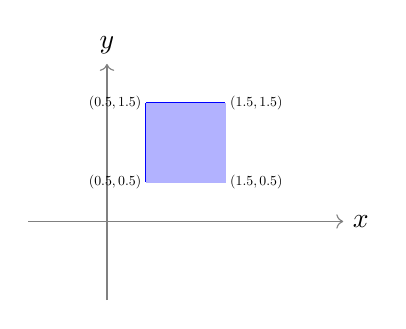
\begin{tikzpicture}
    \draw [thin, gray, ->] (0,-1) -- (0,2)      % draw y-axis line
        node [above, black] {$y$};              % add label for y-axis

    \draw [thin, gray, ->] (-1,0) -- (3,0)      % draw x-axis line
        node [right, black] {$x$};              % add label for x-axis

    \draw [draw=blue,thick] (0.5,0.5) -- (0.5,1.5)% draw the graph
   	 	node [left, black, scale =0.5] {$(0.5,1.5)$};
    \draw [draw=blue,thick] (0.5,1.5) -- (1.5,1.5)
    	node [right, black, scale =0.5] {$(1.5,1.5)$};
    \draw [draw=blue,thick] (1.5,1.5) -- (1.5,0.5)
    	node [right, black, scale =0.5] {$(1.5,0.5)$};
    \draw [draw=blue,thick] (1.5,0.5) -- (0.5,0.5)
    	node [left, black, scale =0.5] {$(0.5,0.5)$};
    	
    \draw [fill=blue!30,blue!30] (0.5,0.5) rectangle (1.5,1.5); 




\end{tikzpicture}
\end{center}
We can represent this information in two different possible ways.
\subsection{Constraint representation}
In constraint representation we model the polyhedron as the intersection of a finite number of closed half spaces and a finite number of subspaces. The resulting polyhedron can be written as:

\begin{equation}
	P=\{x\in Q^n |Ax\leq b \wedge Dx=e\}
\end{equation}
where A,D are matrices and b,e are vectors of natural numbers. Therefore, the constraint representation of the above example would be:

\begin{equation}
	C = \{-x \leq -0.5,x\leq 1.5 , -y \leq -0.5 ,y\leq 1.5\}
\end{equation}

\subsection{Generator representation}
In order to encode a Polyhedron with the generator representation, we have to model it as the convex hull of three items: 

%TODO finish list with rep 
\begin{itemize}
	\item A finite set $V\in Q^n$ of vertices $v_i \in V$.
	\item A finite set $R \subseteq Q^n$ of rays. $r_i \in R$ are direction vectors of infinite edges of the polyhedron with one end bounded. Each ray starts from a $v \in V$.
	\item  A finite set $Z \subseteq Q^n$ of lines. $z_i \in Z$ are direction vectors of infinite edges of the polyhedron with both ends unbounded. Each line passes through a $v \in V$.
\end{itemize}
%TODO finish example
The result of generator representation on the previous example would have the following form: 
\begin{equation}
	G = \{ V = \{(0.5,0.5),(1.5,0.5),(1.5,1.5),(0.5,1.5)\}, R = \emptyset, Z = \emptyset \}
\end{equation}
\subsection{Polyhedra domain}

Now that we can represent our Polyhedra we can do some interesting calculations with them. The polyhedra abstract domain consists of the polyhedral lattice:
	$(P,\sqsubseteq,\sqcup,\sqcap,\perp,\top)$, and a set of operators that we can apply on them. The different operators are the following:
	\begin{itemize}
		\item Inclusion test: $P \sqsubseteq Q$
		\item Equality test: $P=Q$
		\item Join: $P\sqcup Q$
		\item Meet: $P\sqcap Q$
		\item Widening, this operator is applied to accelerate convergence since the polyhedral lattice has infinite height:
		\begin{center}
		  \[
    C_{P\nabla Q}=\left\{
                \begin{array}{ll}
                  C_Q $ if $P=\perp ;\\
                  C'_P\bigcup C'_Q, $ otherwise$;
                \end{array}
              \right.
  	\]
		
		\end{center}

		where $C'_p=\{c\in C_P |C_Q \vdash c \}$, and\\  $C'_Q=\{c\in C_Q |\exists c' \in C_P,C_P \vdash c $ and $((C_P\c')\bigcup \{c\})\vdash c' \}$
		where $C\vdash c$, tests wether c can be entailed from constraints in C
		\item Conditional: let $\otimes \in \{\leq,=\},1\leq 1\leq n,\alpha \in Q$ then $\alpha x_i \otimes \delta$ adds the constraint $(\alpha-a_i)x_i \otimes\delta - a_i x_i$ to the constraint set C
		\item Assignment: $x_i = \delta$, first adds $x_i$ to P then augments C with $x_i -\delta = 0$
		
	\end{itemize}
	 In the following table we can see the respective complexities of the different operators according to the representation
	 
\begin{center}
\begin{tabular}{||c c c c||} 
 
 \hline
 Operator & Constraint & Generator & Both \\ [0.5ex] 
 \hline
 Inclusion $(\sqsubseteq)$ & $O(mLP(m,n))$ & $O(gLP(g,n))$ & $O(ngm)$ \\ 
 \hline
 Join $(\bigsqcup)$ & $O(nm^{2^{n+1}})$ & $O(ng)$ & $O(ng)$ \\
 \hline
 Meet $(\sqcap)$ & $O(nm)$ & $O(ng^{2^{n+1}})$ & $O(nm)$\\
 \hline
 Widening $(\bigtriangledown)$ & $O(mLP(m,n))$ & $O(gLP(g,n))$ & $O(ngm)$ \\
 \hline
 Conditional & $O(n)$ & $O(ng^{2^{n+1}})$ & $O(n)$ \\ 
 \hline
 Assignment & $O(nm^2)$ & $O(ng)$ & $O(ng)$ \\ 
 
 
 \hline
\end{tabular}
\end{center}
$m=|C|,g=|G|,LP(m,n)$ is the complexity of solving a linear program with m constraints and n variables\\
As we can see no representation is less complex than the other, as some of the operators are faster in one but others in the other. But, as we can see in the last table, when both representations are available all the operators have a polynomial complexity.\\
\paragraph{Chernikova's Algorithm} \mbox{}\\
 The first optimisation that one can do is to keep both representations of the the polyhedron and for each operator pick the representation that minimises the time complexity. A conversion between the two representations is possible thanks to Chernikova's algorithm\cite{chernikova1968algorithm}. 
 
 \section{Polyhedra Decomposition}
Another technique used to increase the efficiency of polyhedra analysis, is the use of online decomposition \cite{singh2017fast}. It is based on the observation that during the execution of a program, not all it's variables are dependent on one another. Using this observation, we can separate the set of all variables into smaller, independent sets. Therefore, instead of having to represent the whole set of variables with one large polyhedron we can instead represent it with various smaller ones.\\ Let's assume we have a set of variables $\chi$ in a Polyhedron $P$. The set $\chi$ can be partitioned as $\pi_P=\{ \chi_1,\chi_2,..,\chi_r\}$, $\chi_i\subseteq\chi $. We call the partitioning of the set permissible iff $ \chi_i \cap \chi_j = \emptyset$, $ \forall i \neq j$. We call the $\top$ partition, a partition where all the variables are in one block, i.e no partitioning is done. Similarly, the $\perp$ partition, is a partition where each variable has its own block, i.e all variables are independent of one another. Once the decomposition has been done in this way, during the execution of an operator, it only has to be executed on the subset of blocks that contain it. This allows for a very large performance gain in both space and time, giving us the following time complexity for the various operators.

\paragraph{Table 2} Asymptotic time complexity of Polyhedra domain operators with decomposition

\begin{center}
\begin{tabular}{||c c||} 
 
 \hline
 Operator & Decomposed  \\ [0.5ex] 
 \hline
 Inclusion $(\sqsubseteq)$ & $O(\sum_{i=1}^r n_ig_im_i)$\\ 
 \hline
 Join $(\bigsqcup)$ & $O(\sum_{i=1}^r n_i g_i m_i + n_{max} g_{max})$ \\
 \hline
 Meet $(\sqcap)$ & $O(\sum_{i=1}^r n_i m_i)$ \\
 \hline
 Widening $(\bigtriangledown)$ & $O(\sum_{i=1}^r n_i g_i m_i)$\\
 \hline
 Conditional & $O(n_{max})$ \\ 
 \hline
 Assignment & $O(n_{max}g_{max})$ \\ 
 
 
 \hline
\end{tabular}
\end{center}

 
\paragraph{Example 3.2} \mbox{}\\
Let's consider the variables $X = \{x_1,x_2,x_3,x_4\}$ and $C = \{ x_1 + 2 \cdot x_3 \leq 10, x_2 = 1 \}$.\\
This polyhedron can be partitioned into three blocks $\pi_P = \{\{x_1,x_3\},\{x_2\},\{x_4\}\}$ and its corresponding factors are equal to:
\begin{center}
	$C_{P_1}\{x_1 + 2\cdot x_3 \leq 10 \} , C_{P_2}\{x_2 = 10 \}$
\end{center}

% TODO write example

\subsection{Decomposition operators}
As we change the model of our domain we must equally update the operators inside of this domain. For sake of brevity I will not go into detail about each of them, but I will talk about the join operator as it plays an important role for this paper.\\
During the join of $P$ and $Q$, most of the time their factors will not be equal$(\pi_P \neq \pi_Q)$. Unfortunately, in order to be able to perform the join these must be equal. 
 Therefore, we have to remake their partitions so that $\pi = \pi_P\sqcup\pi_Q$. During most joins of a normal execution this will not cause much problem, but during some cases the join can merge all blocks $(\pi_P\sqcup\pi_Q = \top)$ producing the $\top$ partition. In order to rebuild the $\top$ partition from the factors we use the following formula:
\begin{equation}
	P = P_1 \Join P_2 \Join ... \Join P_r = (C_{P_1} \cup C_{P_2} \cup ... \cup C_{P_1}, G_{P_1} \times G_{P_2} \times  ... \times   G_{P_r})
\end{equation}
Due to the cartesian product, building the $\top$ partition can blow up the number of generators and cause the join to be a serious bottleneck of online decomposition.

\section{Reinforcement Learning for polyhedra analysis}
Both of the techniques presented in chapters 3.2 and 3.3, manage to achieve considerable performance gain without having to sacrifice any precision. Unfortunately, at some point compromises have to be made. Analysers that tune the precision and cost based on the program they are analysing are called parametric program analysers. Several such approaches already exist. \cite{oh2015learning,liang2011learning,heo2016learning}.
As explained in 3.3.1. one bad constraint can significantly decrease the performance of the whole program. The trick is being able to identify this constraint at the correct time. One of the explored solutions to this problem that we shall explore, is training a reinforcement learning algorithm  that will make the decisions of when and how to apply some abstractions\cite{singh2018fast}.\\
Intuitively, using reinforcement learning for polyhedra analysis seems quite straight forward. Let's imagine that for the join operator that we have presented above, we have two different versions $J_{pr}$ and $J_{pe}$. One of these is a slower and more precise join and the other, using some sort of abstraction, is faster but not as precise. The goal of the reinforcement learning method would then simply be to select the correct operator at the right time, so that we get the most precise result in as little time as possible. Before this can be done, it is first necessary to initialise polyhedra analysis for reinforcement learning.

\subsection{Adapting polyhedra analysis for Reinforcement Learning}
As explained in 2.1., reinforcement learning uses a defined set of concepts. In some way, these concepts have to be translated into the domain of polyhedra analysis. A possible mapping can be done in the following way.
\begin{center}
\begin{tabular}{||c c||} 
 \hline
 RL concept & Polyhedra analysis concept  \\ [0.5ex] 
 \hline
 \hline
 Agent & Static analyser\\ 

 State $s\in S$ & some features describing the polyhedron\\

 Action $a \in A$ & Abstract transformer \\
 
 Reward function r & some function representing the runtime\\
 
  & and precision of a polyhedron\\
 \hline
\end{tabular}
\end{center}
A more concrete explanation of the initialisation of these concepts will come in the following chapter.

\subsection{Linear function approximation methods}
Existing methods already exploit this idea \cite{singh2018fast}. Using techniques such as Q-learning in order to learn their decision making policies. Q-learning is a common linear Q-function approximation technique that has shown some very good results when applied to the polyhedra domain.\\
However, recently, new reinforcement learning methods seem to be more focused on the use of nonlinear Q-function approximators, as they seem to give very good results on some  complex tasks. When the Q-function of the particular problem is nonlinear, Q-learning will never be able to learn the ideal policy. In these cases, deep Q-networks have a very real opportunity of exceeding the performance of the Q-learning based methods.\\
The use of nonlinear approximators has not yet been tested on the domain of static analysis. In the following chapters we shall explore the idea of using such methods in order to construct a new decision policy based on neural networks.

















% !TEX root = ../thesis.tex

\chapter{Fast polyhedra analysis with deep Q-networks}
\mbox{}\\
The goal of my work was to build upon the existing solutions, used to make polyhedra analysis more efficient and use deep Q-networks to further improve the performance. Specifically, my goal was to extend the Elina Framework, the version of it that used reinforcement learning for polyhedra analysis, in order to use deep Q networks for the Q function estimation. The work I have done can be separated into three major subtasks. First of all, I had to figure out a way of calling a deep neural network form Elina \cite{elina}, so that I could use it for the Q function estimation. Secondly, In order to test out the validity of deep Q-networks on polyhedra analysis and to have a baseline for further optimisation. I implemented the basic deep Q-network training algorithm. Finally, I attempted to further optimise this problem with some task specific knowledge.
\section{Incorporating Neural Networks inside Elina}
The first part, whilst definitely being the least interesting was probably the most laborious and a very key part of the whole work. The problem was that for my Q value estimation I wanted to use neural network regression from Keras in Python. I decided to use this framework as it is very widely used for this type of problem, is relatively easy and intuitive to use whilst remaining very powerful. However, Elina being written in C, I somehow had to make the link between my Python code and the C code of Elina. I finally achieved this by using the Python/C API and embedding the python code into the Elina framework. Initialising all the python code as well as importing all the necessary libraries such as Keras, is done in the $op\_pk\_manager\_alloc()$ function so that it doesn't have to be done every time we call the join function. Inside the join function we simply have to call the learning or prediction algorithms.\\
One advantage of such a modification to the framework, is that we can now learn online. In comparison to \cite{singh2018fast} which did its training offline. Online training allows the algorithm to pick the best action according to the current decision policy. This is a very important feature for deep Q-networks, as it allows us to set an exploration rate and to reinforce the already learned policy, this is vital to prevent divergence.
\section{Basic algorithm}
In order to get the basic training algorithm working, first the domain of polyhedra analysis has to be made compatible with the domain of reinforcement learning. Therefore the following list of items have to be initialised inside of the polyhedra domain:
\begin{itemize}
	\item A set of features describing the polyhedra to use as states $S$
	\item A set of actions $A$
	\item A reward function $r$
\end{itemize}
Luckily, since a reinforcement learning method \cite{singh2018fast} has already been used for polyhedra analysis we can simply reuse what has already been developed for our baseline algorithm.\\
\subsection{Features}
The reinforcement learning method used a set of nine different features.
\begin{itemize}
	\item The number of blocks.
	\item The minimal, maximal and average size of a block.
	\item The minimal, maximal and average size of the generator set off the union of input factors corresponding to a block.
	\item The number of variables with finite upper and lower bound.
	\item The number of variables with one finite and one infinite bound.
\end{itemize}
We will reuse the same features for the baseline algorithm. However we will modify their bucketing, since, due to the nature of the Q-learning method, it is very restrictive. The new bucketing will be discussed in section 4.3.2.

\subsection{Actions}
As we discussed in 3.3.1., the bottleneck of the decomposed analysis is the join. Therefore, the set of actions will be a various set of joins of different precision and performance.\\
First of all, the cost of the joins depends on the size of the block. Therefore, bounding the the size of the block with a threshold would increase the performance. These four different thresholds are used $threshold \in [5,9],[10,14],[15,19],[20,\infty)$\\
Once we have decided on the size of a threshold we have to equally decide on what to do if the block has a greater size than the threshold. Their are different possibilities of how to split a large block into smaller ones, but basically, one has to pick a subset of constraints to remove from the block so that all its constraints are no longer dependant and then it can be further partitioned. The following three constraint removals are used:
\paragraph{Stoer-Wagner min-cut}\mbox{}\\
This algorithm is based on the simple idea of removing the minimal amount of constraints in order to be able to split to block into two separate permissible partitions \cite{stoer1997simple}.
\paragraph{Weighted constraint removal}\mbox{}\\
The second and third constraint removal techniques are based on the same principal. They associate a certain weight to each constraint  and then remove the constraint with the highest weight. Two different weight distribution techniques are considered. \\
In the first one, we first compute for each variable $x_i \in X$ the number of constraints it appears in, we can call this $n_i$. Then for each constraint $c_i$ we set its weight to the sum of $n_i$ of all the variables that are in the constraint.\\
The second method, we first compute for each pair of variables $x_i,x_j\in X$, $n_{ij}$ the number of constraints containing both $x_i$ and $x_j$. The weight of the constraint is then the sum of all the $n_{ij}$ of all the pairs of constraints $x_i,x_j$ contained in the constraint.\\
The idea of removing the constraint with maximal weight, is that, most likely the variables occurring in the constraint are also bounded by other constraints and therefore will not become unbounded once the constraint is removed.
\paragraph{Merging blocks}\mbox{}\\
The next three actions are various block merging strategies. The idea is to select different blocks and merge them together as long as the resulting blocks remain below the threshold in order to increase the precision of the subsequent join. The following three block merging strategies are used:
\begin{itemize}
	\item No merge, no blocks are merged
	\item Merge smallest first, we first merge the smallest two blocks together. We then remove the smallest block and continue as long as the resulting merge remains below the threshold.
	\item Merge small with large, similar to the previous strategy but this time me merge the smallest block with the largest.
\end{itemize}

In total we have four different thresholds, three different constraint removal algorithms and three different block merging strategies. We can mix and match these together as we please, which means that in total we have $4\times 3\times 3 =36$ different actions we can pick.



Once this has been done, I could finally proceed to the more interesting part of writing the training algorithm. Under its most basic form, the training algorithm could simply be the following. Pick a random reward or maximal action, observe the reward and then retrain the network with the observed plus the discounted  future reward on the given action. This very basic algorithm however did not get me very far as I ran into two main problems.
\subsection{Reward}
As a reminder, the objective of the reward is to guide our learning policy. Rewarding it when it takes actions towards our global goal and penalising it when it does otherwise. Therefore, the reward developed by the Q-learning method was the following:
\begin{equation}
	r(s_t,a_t,s_{t+1}) = 3  \cdot n_s + 2 \cdot n_b + n_{hb} - \log_{10}(cyc)
\end{equation}
Where $n_s$ is the number of exactly defined variables of the resulting polyhedron after the join. $n_b$ is the number of bounded variables and $n_{hb}$ the number of semi-bounded variables of the resulting polyhedron. $cyc$ is the number of cycles required to perform the join.
\subsection{Back to deep Q-networks}
As we have finally initialised polyhedra analysis for the use with reinforcement learning. We can finally proceed to the more interesting part of designing the training algorithm. Under its most basic form, the training algorithm could simply be the following. Pick a random reward or maximal action, observe the reward and then retrain the network with the observed plus the discounted  future reward on the given action. This very basic algorithm however did not get me very far as I ran into two main problems.

\paragraph{Divergence of decision policy}\mbox{}\\
The first of which was the divergence of the action selection strategy. Meaning that neural networks were not able of creating a consistent strategy but would be picking different actions all the time.
\paragraph{Divergence of the action value prediction}\mbox{}\\
The second problem was that the predictions of my estimator would diverge towards infinity. This is also known as the exploding gradient problem.\\
\mbox{}\\
These problems are not new and are a fundamental problem of trying to use non-linear functions for the Q-function approximation. Several techniques exist to combat these problem. Many of which reduce the complexity of the network and or the problem in general. However, some new methods have been developed recently that would allow the training of the estimators whilst retaining the problems original complexity. I decided the use the following two concepts inside of my algorithm.
\subsection{Experience replay memory}
Experience replay memory \cite{Mnih2015} is a biologically inspired mechanism. That gives the estimator a very basic concept of a memory and instead of directly learning from the current events happening. The agent learns from a random subset of its memroy. More formally, during training, an array of a certain size filled with the past memory objects is kept. Each memory item contains the following items: $mem(s_t, a_t, r_t, s_{t+1})$. The current state, the action taken at this state, the observed reward and the next state. For training we then simply pick a random subsample from the memory array and train from these examples.
\\
The objective of the memory is to homogenise the training data. It comes from the observation that during the execution of a program, often a particular strategy would be optimal during a certain period of time and afterwards another one would be the new optimal. This caused two major problems. First of all, it is not very time efficient as we do not gain much information by learning from the same data. Secondly, as there was low diversity in the training data and the decision strategy would frequently abruptly change it. This either led to the neural network getting stuck in local minima or simply to diverge and not obtain a policy. \\
Picking a random subsample from memory helps increase the variance amongst the training data allowing the network to learn a more global policy. 
\subsection{Separating target from max Q estimators}
The other method used to reduce the divergence of the predicted Q values towards infinity, was to reduce the correlation between the training and the prediction data \cite{Mnih2015}. This was done because, since the networks were being fitted based on the maximum Q value estimation, diverging towards infinity reduced their error and therefore was a valid strategy that they would use. In order to reduce this correlation, the networks predicting the maximum Q value and the ones predicting the Q value were separated. The weights of the maximum Q-value estimators were then updated every n steps in order for them to remain up to date.\\
\mbox{}\\
Further modifications were also made on the neural network level in order to reduce these problems. I will get into these in part.\\
%TODO add part
Once these modifications have been made the basic training algorithm has the following form.
\paragraph{Pseudo code of basic learning algorithm}

\begin{center}
	
\begin{algorithm}[H]
    \SetKwInOut{Input}{Input}
    \SetKwInOut{Output}{Output}

    \textbf{function} \text{learn} $(S,A,r,\gamma,\alpha,\phi,N,l\_freq,b\_size,update\_nn\_freq,\varepsilon)$\;
    
    
    \Indp\Input{\\$S \leftarrow states, A \leftarrow Actions, r \leftarrow reward,$\\$ \gamma \leftarrow discount$ $factor, \alpha \leftarrow learning$ $rate,$\\$\phi \leftarrow$ set of feature functions over S and A \\ N $\leftarrow$ size of memory, l\_freq$\leftarrow$ learning frequency,\\ b\_size $\leftarrow$ batch size, $\varepsilon \leftarrow$ random action probability,\\ update\_nn\_freq $\leftarrow$ frequency of updating max Q estimators}\Indm
    \Indp\Output{\\$\theta \leftarrow$ trained weights of the estimator}\Indm
    \Indp
    $\theta = $ initialise random weights and learning rate $\alpha$\\
    $\theta_{max} = $ initialise random weights and learning rate $\alpha$\\
    $M = $ initialise an empty memory with size N\\
    
    \For{each episode}{
    start from initial state $s_{_0} \in S$\\
    \For{$t=0,1,2,...$}{
    Initialise new memory item $m_t$\\
    With probability $\varepsilon$ take random or maximal action $a_t$\\
	observe next state $s_{t+1}$ and
     $r_{t}(s_{t},a_t,s_{t+1})$\\
     Set $m_t.a = a_t,m_t.s_1=s_{t},m_t.s_{2}=s_{t+1},m_t.r=r_{t}$ \\
     
     \Indm
     \Indp\uIf{$M_{size} \geq N$}{
    	del $M_0$ \\
     	$M_{N}=m_t$
		}
		\uElse{
		push $m_t$ on M
	}\Indm
	\Indp\uIf{$t\mod l\_freq = 0$}{
	select a random batch of size b\_size from m\\
	compute $Q(:,s_t)$ estimation with $\theta$\\
	compute $Q(:,s_{t+1})$ estimation with $\theta_{max}$\\
	set $Q(a,s_t) = Q(a,s_t) + \gamma*max(Q(:,s_{t+1}))$\\
	Fit weights $\theta$ with new training data
	}\Indm
	\Indp\uIf{$t\mod update\_nn\_freq = 0$}{
	set $\theta_{max} = \theta$
	}
			
    }
    
   }
   \textbf{return} $\theta$
    
\caption{DQN Training algorithm}
\end{algorithm}
\end{center}
\mbox{}\\
\mbox{}\\
\mbox{}\\

\section{Further optimisations}
Once the basic version of the deep Q-network algorithm was designed we were able to train it, test it and obtain our first set of results. The discussion of these will be done in chapter 5. These results can from now on be used as a benchmark and we can try to further improve our results.\\
In the search of a more efficient algorithm, we decided to incorporate some problem specific knowledge to the deep Q-network algorithm. As well as further optimisations to the feature vector and reward functions. The modifications made will be discussed in the rest of this section.


\subsection{Separating the problem into two}
The first problem specific modification I made, was subdividing the problem into two independent subproblems. The objective of Polyhedra Analysis is to obtain the most precise result in the quickest way possible. These are two independent objectives. My goal was therefore to separate these two tasks and create two independent subsystems, one focusing on making the results as precise as possible, and the other on the time complexity of getting there.\\
 Such a division of the problem, offer two main advantages. Firstly, a greater flexibility during training. The parameters of each system can be tuned for its specific needs. So for example the characteristics of the neural network or the discount factor. Furthermore, the optimal features used for precision and performance estimation, are quite probably different. The separation therefore allows us to use only the necessary features for each subsystem making the learning and prediction less complex and therefore more precise and converge faster. The reward as well can be fine tuned for the needs of the specific needs of the subsystem.\\ 
 Secondly, two separate subsystems also allow for a more flexible algorithm post training. Since during training, we will have trained two different Q function estimators, during prediction we will have a greater possibility of optimising our results by changing the importance we give to each subsystem at different points in time according to the specific needs. I will get into more detail about this in the section about the action selection policy.\\
 The pseudo code for the training algorithm with separated estimators has the following form:


\paragraph{Pseudo code of the separated training algorithm}
\begin{center}
	
\begin{algorithm}[H]
    \SetKwInOut{Input}{Input}
    \SetKwInOut{Output}{Output}

    \textbf{function} \text{learn} $(S,A,r,\gamma,\alpha,\phi,len,l\_freq,b\_size,update\_nn\_freq)$\;
    
    
    \Indp\Input{\\$S \leftarrow states, A \leftarrow Actions, r \leftarrow reward,$\\$ \gamma \leftarrow discount$ $factor, \alpha \leftarrow learning$ $rate,$\\$\phi \leftarrow$ set of feature functions over S and A \\ len $\leftarrow$ size of memory, l\_freq$\leftarrow$ learning frequency,\\ b\_size $\leftarrow$ batch size,\\ update\_nn\_freq $\leftarrow$ frequency of updating max Q estimators}\Indm
    \Indp\Output{\\$\theta_1 \leftarrow$ trained weights of neural network for performance \\ $\theta_2 \leftarrow$ trained weights of neural network for precision}\Indm
    \Indp
    $\theta_1 = $ initialise random weights\\
    $\theta_2 = $ initialise random weights\\
    $\theta_{1\_max} = $ initialise random weights\\
    $\theta_{2\_max} = $ initialise random weights\\
    $m = $ initialise an empty memory\\
    
    \For{each episode}{
    start with initial states $s_{pr\_0} \in S, s_{pe\_0} \in S$\\
    \For{$t=0,1,2,...$}{
    Initialise new memory item $m_t$\\
    Take action $a_t$ according to the action selection algorithm \\ observe next state $s_{pr\_t+1},s_{pe\_t+1}$ and
     $r_{pe}(s_{pe\_t},a_t,s_{pe\_t+1}),r_{pr}(s_{pr\_t},a_t,s_{pr\_t+1})$\\
     Set $m_t.a = a_t,m_t.s_{pr\_1}=s_{pr\_t},m_t.s_{pe\_1}=s_{pe\_t},m_t.s_{pr\_2}=s_{pr\_t+1},m_t.s_{pe\_2}=s_{pe\_t+1},m_t.r_{pr}=r_{pr},m_t.r_{pe}=r_{pe}$ \\
     
     \Indm
     \Indp\uIf{$m_{size} \geq len$}{
    	del $m_0$ \\
     	$m_{len}=m_t$
		}
		\uElse{
		push $m_t$ on m
	}\Indm
	\Indp\uIf{$t\mod l\_freq = 0$}{
	select a random batch of size b\_size from m\\
	compute $Q(:,s_t)$ estimation with $\theta_1,\theta_2$\\
	compute $Q(:,s_{t+1})$ estimation with $\theta_{1\_max},\theta_{2\_max}$\\
	set $Q(a,s_t) = Q(a,s_t) + \gamma*max(Q(:,s_{t+1}))$\\
	Fit weights $\theta_1,\theta_2$ with new computations from this batch
	}\Indm
	\Indp\uIf{$t\mod update\_nn\_freq = 0$}{
	set $\theta_{1\_max} = \theta_1,\theta_{2\_max}= \theta_2$
	}
			
    }
    
   }
   \textbf{return} $\theta_1,\theta_2$
    
\caption{DQN Training algorithm}
\end{algorithm}
\end{center}



\subsection{Feature selection}
Before I get into the specific features I used for my estimators, I would like to go a bit more in-depth about the theory of features and states. States in the case of polyhedra analysis would be the concrete Polyhedra. However, during our analysis we do not use the concrete polyhedra as this would be too complicated, but rather some information that we extract from them, we call this the feature vector. As explained in section 2.1., for reinforcement learning, states should respect the Markov property that states that $s_{t+1}$ only depends on $s_t$ and on $a_t$. Whilst this is the case for the polyhedra, our feature vectors do not have to obey this property as they do not represent the polyhedra themselves but only some information about them. The more precisely we manage to describe our polyhedron the closer we will be to respecting the Markov property and the better will be the results of RL. 

With regards to the old set of features. One big inconvenience of using Q-learning, is that, since we want to represent our Q-function with basis functions, the size and dimensions of our feature vector is very limited. This constraint no longer holds when using more advanced methods such as deep Q-networks. This allowed me to make two major changes about the feature vector. 
\paragraph{Adding new features}\mbox{}\\
The first change I was able to make, was to add some new features.First of all, I reused the nine features from the Q-learning algorithm. The first seven features of these features are used to characterise the complexity of the join. They are the number of blocks, minimal, maximal and average size of the blocks and the minimal, maximal and average size of the generator set. The last two features are used to characterise the precision of the inputs and they are the number of variables with a finite upper and lower bound, as well as the number of variables with a finite upper or lower bound, in both Polyhedra.\\
I further extended this set with four new features, in order to further increase the description accuracy of the feature vector. The selection of these features was done by trial and error, with an experimental observation of an increase, or lack thereof, off accuracy. It is also possible to check whether a particular feature is useful once training it finished by analysing the neural network and observing the impact a particular feature has on the end result. However, since at the end my network had a total of four layers, this made its analysis somewhat complicated.\\
At the end I added a total of four new features, three of which are used for modelling the precision and one for the complexity. For the complexity I added the number of constraints. As for the precision I added the number of unconstrained variables, the number of exactly constrained variables and finally, the sum of the values the bounded variables can have (i.e. an approximation of the circumference of the polyhedra). I also tried using some features that would have perhaps modelled the precision more accurately, such as most notably approximating the volume of the polyhedra. Unfortunately, one must also consider the complexity of computing the features. The computation of the volume approximation was far too time complex, which greatly increased the learning time making the feature not viable.\\
\paragraph{Bucketing}\mbox{}\\
Due to the limitations of Q-learning the old algorithm used a very restrictive bucketing policy. Deep reinforcement learning does not suffer from these restrictions. I was therefore able to remove the bucketing from the feature selecting. I still implemented a version of bucketing in my algorithm for three main reasons. \\
Firstly, for features with very big values an exact precision is not needed. For example, for the feature that approximates the circumference of the polyhedra, its total value can be very big and and if it is a million and one or just a million doesn't impact the resulting precision much therefore bucketing makes sense. \\
The second reason, for the use of bucketing is that it greatly decreases the learning time and helps convergence. \\
Finally, the last reason is that the decision policy doesn't give more importance to some features simply because they are larger than others. In my total of thirteen different features, they all can have very different values. For example, the number of blocks varies mainly between one and ten, and the circumference of the polyhedra can go up to $10^9$. This does not mean that the circumference has a greater impact on the overall precision of the polyhedra. Bucketing assures that all features have a similar impact on the decision policy.\\
In order to decide the values of the bucketing I would use, I ran my algorithm on a big number of benchmarks computing the maximal, minimal and average values the different features could have. Finally, I scaled them so that they would all approximately remain between the bounds of zero and ten. I then bucketed them in the following fashion:
\begin{center}

\Indm\Indm\begin{tabular}{||c c c c||} 
 
 \hline
 Feature & Extraction complexity & Approximate range & Scaling \\ [0.5ex] 
 \hline\hline
 $|\beta|$ & $O(1)$ & 1-10 & $x/1.$ \\ 
 \hline
 $min(|\chi_k|:\chi_k \in \beta)$ & $O(|\beta|)$ & 1-50 & $round((x/5),0.5)$ \\
 \hline
 $max(|\chi_k|:\chi_k \in \beta)$ & $O(|\beta|)$ & 1-50 & $round((x/5),0.5)$ \\
 \hline
 $avg(|\chi_k|:\chi_k \in \beta)$ & $O(|\beta|)$ & 1-50 & $round((x/5),0.5)$ \\
 \hline
 $min(|\bigcup G_{P_{m}}(\chi_k)|:\chi_k \in \beta)$ & $O(|\beta|)$ & 1-10000 & $round((x/1000),0.1)$ \\ 
 \hline
 $max(|\bigcup G_{P_{m}}(\chi_k)|:\chi_k \in \beta)$ & $O(|\beta|)$ & 1-10000 & $round((x/1000),0.1)$ \\ 
 \hline
 $avg(|\bigcup G_{P_{m}}(\chi_k)|:\chi_k \in \beta)$ & $O(|\beta|)$ & 1-10000 & $round((x/1000),0.1)$ \\ 
 \hline
 $\{|x_i \in X: x_i \in (-\infty,\infty)$ in $P_m|\}$ & $O(ng)$ & 1-100 & $round((x/10),0.5)$ \\ 
  \hline
 $\{|x_i \in X: x_i \in [l_m,\infty)$ in $P_m|\} + $ & $O(ng)$ & 1-50 & $round((x/5),0.5)$ \\ 
 $ \{|x_i \in X: x_i \in (-\infty,u_m]$ in $P_m|\} $ & & & \\
 \hline 
 $\{|x_i \in X: x_i \in [l_m,u_m]$ in $P_m|\}$ & $O(ng)$ & 1-50 & $round((x/5),0.5)$ \\ 
   \hline
 $\{|x_i \in X: x_i \in [u_m,u_m]$ in $P_m|\}$ & $O(1)$ & 1-200 & $round((x/20),0.2)$ \\ 
    \hline
 $|X|$ & $O(ng)$ & 1-50 & $round((x/5),0.5)$ \\ 
    \hline
 $\sum (u_m-l_m):u_m,l_m \in\{[l_m,u_m]$ in $P_m \}$ & $O(ng)$ & $2*10^9$ & $round((x/2*10^8),0.01)$ \\ 
 
 
 \hline
\end{tabular}
\end{center}
One thing to note is, that as opposed to the reinforcement learning algorithm, my features do not have a maximal possible value. I believe that this increases the precision of the q function estimation, especially for the approximation of the complexity. Certain features can have very large values and I believe when this arrives, it has a major impact on the complexity of the join. However, these very large values were ignored by the bucketing of the reinforcement learning algorithm. 

\subsection{Reward Function modelling}
Due to the nature of the new algorithm, the modelling of the reward function was separated into two separate subproblems.
\paragraph{Performance reward}\mbox{}\\
Firstly, the reward for the precision estimator and then the reward for the performance estimator. Modelling the complexity is fairly simple and very straight forward, as simply counting the number of cycles needed for the computer to execute the join perfectly models the complexity and is exactly what we want to optimise. One thing to note is that we want this reward to be as small as possible, two simple solutions for this are either to invert it or to negate it. I experimented with both of these and found that negating it produces better results. I assume this is due to the fact that inverting the reward, makes it have a nonlinear curve and its derivative looses importance the higher the CPU cycles are, which is not something we want. Another thing to note is that modelling the complexity reward in this way give us another advantage over the reinforcement learning version of the algorithm. The reinforcement learning algorithm took the $\log_{10}$ off the CPU Cycles in order for the complexity and the precision reward to have similar values. I believe that this produces a similar problem as inverting the reward. The reward is no longer linear and its differences loose importance the higher it gets. Once again, this is not something that we want to model. The final rewards has the following form:
\begin{equation}
	r_{pe}(s_t,a_t,s_{t+1}) = -1 \cdot cyc
\end{equation}
Where $cyc$ is the number of CPU cycles.
\paragraph{Precision reward}\mbox{}\\
As to the second reward, modelling the precision of the resulting join. This is considerably more difficult than modelling the complexity as there is no trivial element giving us the precision of our polyhedron. In order to choose the reward, I proceeded by intuitively picking a small set of options and verifying them experimentally at the end. At the end, I tested out three different reward.\\
I took the first one from the reinforcement learning algorithm, that is, the objective is to maximise the amount of exactly bounded, bounded and half bounded variables. The second is a further extension by penalising the amount of values a bounded variable can have in the resulting Polyhedra. The final, reward function is slightly different. In this one, I penalise the loss of an exactly bounded, bounded or half bounded variable. Reward the loss of a bounded variable and penalise the amount of values a bounded variable can have. I also tried basing a reward function on an approximation of the volume of the resulting Polyhedra, unfortunately, the complexity of this computation was too high which made it too impractical to use in practice. The final rewards have the following form:
\begin{equation}
		r_{pr_1}(s_t,a_t,s_{t+1}) = 3  \cdot n_s + 2 \cdot n_b + n_{hb}
\end{equation}
\begin{equation}
		r_{pr_2}(s_t,a_t,s_{t+1}) = 3  \cdot n_s + 2 \cdot n_b + n_{hb} - \log_{10}(|n_b|)
\end{equation}
\begin{equation}
		r_{pr_3}(s_t,a_t,s_{t+1}) = 3  \cdot (n_{s_f} - n_{s_i}) + 2 \cdot (n_{b_f} - n_{b_i}) + (n_{hb_f} - n_{hb_i}) - \log_{10}(|n_b|)
\end{equation}\mbox{}\\
Where $n_s$ is the number of exactly defined variables of the resulting polyhedron after the join. $n_b$ is the number of bounded variables and $n_{hb}$ the number of semi-bounded variables of the resulting polyhedron. $n_{x_f}$ is the number of variables after the join and $n_{x_i}$ before the join.
\subsection{Action selection algorithms}
As discussed before, I separated the Q function estimation into two separate subproblems. As I already mentioned earlier, this allows a certain amount of benefits that would not be possible otherwise. However, it also imposes one major complication. These two problems are not totally separable, as once we have predicted the two q function estimations, we have to somehow merge the information contained in both of these estimations and pick an ideal action accordingly. I tried out a few different action selection algorithms in order to find the one that maximises precision and performance the most. One thing to note is that it is at least partially possible to test out these algorithms post training. That is to say that we do not have to train using these in order to measure their performance afterwards. This only works if we train purely randomly however. As if, if we were to train using one selection algorithm and then test with another, this would surely deteriorate the results. The fact that we are able to test the selection algorithms after random training is still very helpful as the training time is relatively high and having to train for each algorithm would be very time intensive.
\paragraph{Algorithm 1}\mbox{}\\
The first selection algorithm I used is perhaps the most intuitive one. First scaling both q function estimations. The performance one between [-1,0] and the precision one between [0,1]. Adding the values together and picking the action with the maximal value. Whilst seeming very fair this type of selection has a couple of fundamental flaws. First of all, reinforcement learning estimates the best action to take in order to maximise the long-term objective, it however has less of a guarantee about the second to best and third to best action. This means that if the network is well trained, the chances that the action with the maximal Q-value prediction is also the best action to take at this point in time should be quite high. However, the guarantee that the action with the second highest Q-value prediction is the second-best action to take is much smaller. Using this selection algorithm tends to quite often not choose the best action but the second best or the third etc... making the probability that they are also good actions also a lot smaller. The second problem with this type of selection algorithm is that scaling the reward function causes a loss of information that could be very important. I will demonstrate this with an example, let's say we have four joins j1,j2,j3,j4. J1 takes one second, j2 ten seconds, j3 one hour and j4 ten hours. Let's also say that j1 and more precise than j2 and j3 is more precise than j5. This algorithm is going to treat the difference between j1 and j2 the same as the one between j3 and j4, even though the gain in precision might be worth to loss in performance for the case of j1 and j2, whilst this would probably not be case for j3 and j4.
\paragraph{Pseudo code of algorithm 1}
\begin{center}
\begin{algorithm}[H]
    \SetKwInOut{Input}{Input}
    \SetKwInOut{Output}{Output}

    \textbf{function} \text{select1} $(Q_{pr},Q_{pe})$\;
    
    
    \Indp\Input{\\$Q_{pr}\leftarrow$array of Q-function estimations for precision,\\$Q_{pr}\leftarrow$array of Q-function estimations for performance}\Indm
    \Indp\Output{\\$a \leftarrow$ action to take} \Indm
    \Indp
    $Q_{pr} = Q_{pr}/max(Q_{pr})$\\
    $Q_{pe} = Q_{pe}/min(Q_{pe})$\\
    $a = max_{arg}(Q_{pr}+Q_{pe})$
    
  
   \textbf{return} $a$

\caption{Action selection algorithm 1}
\end{algorithm}
\end{center}
\paragraph{Algorithm 2}\mbox{}\\
The second algorithm used, that directly confront both problems of the previous algorithm proceeds as follows. We set some sort of threshold for the performance. We then look at the action that has the maximal Q-value for precision. If this actions Q-value for performance is above the threshold we take it otherwise we take the second-best action and continue until we find an action that is above the threshold. Again, this algorithm seems quite good at first glance and maybe if it was executed perfectly it would be the best option, but like the one before it has some fundamental problems. First of all, picking a threshold is not a very simple task. The q function estimator is a regression neural network, the activation function of its last layer is linear, this means that the output values are unbounded and they do not have a direct correlation with Realtime CPU cycles. In order to pick a threshold, I had to experimentally try different possible values and observe the resulting precision and adjust accordingly, however this threshold would vary according to the benchmark and therefore choosing an optimal one was a very difficult task on its own. Another problem of this algorithm is that If no action has a q performance estimation above the threshold the algorithm will choose the action with the worst precision, and this one does not even have to have the best performance estimation. 
\paragraph{Pseudo code of algorithm 2}
\begin{center}
	\begin{algorithm}[H]
    \SetKwInOut{Input}{Input}
    \SetKwInOut{Output}{Output}

    \textbf{function} \text{select2} $(Q_{pr},Q_{pe},PE_{thresh})$\;
    
    
    \Indp\Input{\\$Q_{pr}\leftarrow$array of Q-function estimations for precision,\\$Q_{pr}\leftarrow$array of Q-function estimations for performance,\\ $PE_{thresh}\leftarrow$performance threshold}\Indm
    \Indp\Output{\\$a \leftarrow$ action to take} \Indm
    \Indp
    \While{$max(Q_{pr})\neq 0$}{
    a = $max_{arg}(Q_{pr})$\\
    \uIf{$Q_{pe}(a)\geq PE_{thresh}$}{
    break;
    }
    $Q_{pr}(a)=0$
    }
    
   
  
   \textbf{return} $a$
   
    
\caption{Action selection algorithm 2}
\end{algorithm}
\end{center}
\paragraph{Algorithm 3}\mbox{}\\
Another possibility is to slightly modify the previous algorithm in order to minimise some of its short comings. This time we set both some sort of a threshold for the performance and a certain number x. if the action that has the highest precision estimation is under the threshold for performance, we take the x best actions according to their precision and take the one that has the highest performance estimation. The problem of picking an appropriate threshold remains the same and this time we have the further problem of picking a correct value for x. However, the case that all actions are under the threshold is no longer a problem. It is worth noting that this algorithm also has a greater time complexity, however this is still greatly outweighed if the correct action is taken.
\paragraph{Pseudo code algorithm 3}
\begin{center}
	\begin{algorithm}[H]
    \SetKwInOut{Input}{Input}
    \SetKwInOut{Output}{Output}

    \textbf{function} \text{select3} $(Q_{pr},Q_{pe},PE_{thresh},N_{act})$\;
    
    
    \Indp\Input{\\$Q_{pr}\leftarrow$array of Q-function estimations for precision,\\$Q_{pr}\leftarrow$array of Q-function estimations for performance,\\ $PE_{thresh}\leftarrow$performance threshold, \\$N_{act}\leftarrow$number of actions to consider if below threshold}\Indm
    \Indp\Output{\\$a \leftarrow$ action to take} \Indm
    \Indp
   	$a=max_{arg}(Q_{pr})$\\
   	\uIf{$Q_{pe}(a)\leq PE_{thresh}$}{
   		$a_{max}=a$\\
   		$val_{max}=Q_{pr}(a)$\\
   		$Q_{pr}(a)=0$\\
   		\For{$i \in N_{act}$}{
		   	$a=max_{arg}(Q_{pr})$\\
		   	\uIf{$Q_{pe}(a)\geq val_{max}$}{
		   		$a_{max}=a$\\
		   		$val_{max} = Q_{pe}(a)$
		   	}
		   	$Q_{pr}(a) = 0$
   		}
   	}
    
   
  
   \textbf{return} $a_{max}$
   
    
\caption{Action selection algorithm 3}
\end{algorithm}
\end{center}
\paragraph{Algorithm 4}\mbox{}\\
Finally, the last selection algorithm that I will talk about here is based upon the last one and made in such a way as to reduce the importance of correct parameter choosing. This time we begin by scaling the performance prediction to [-1,0]. We set a threshold to [0,1]. We pick the action that has the highest precision q estimation. If the absolute value of this action's performance estimation minus the maximal performance estimation is below the threshold, then we pick this action otherwise we pick the second-best precision action until we find one that is below the threshold. This time, since we compare to the best performance action we are guaranteed to be below the threshold at some point, in the worst case we will pick the action with the best performance. The threshold is also a lot easier to set since it is bounded. Unfortunately, once again we have the problem caused by the scaling of the performance estimation. However, after some experimental observation, I saw that when the join is fast all the q performance estimations tend to be quite close together, so hopefully this will not be all too much of a problem.
\paragraph{Pseudo code algorithm 4}
\begin{center}
	\begin{algorithm}[H]
    \SetKwInOut{Input}{Input}
    \SetKwInOut{Output}{Output}

    \textbf{function} \text{select4} $(Q_{pr},Q_{pe},PE_{thresh})$\;
    
    
    \Indp\Input{\\$Q_{pr}\leftarrow$array of Q-function estimations for precision,\\$Q_{pr}\leftarrow$array of Q-function estimations for performance,\\ $PE_{thresh}\leftarrow$performance threshold}\Indm
    \Indp\Output{\\$a \leftarrow$ action to take} \Indm
    \Indp
    $Q_{pr} = Q_{pr}/max(Q_{pr})$\\
    $Q_{pe} = Q_{pe}/min(Q_{pe})$\\
	\While{$True$}{
		$a=max_{arg}(Q_{pr})$\\
		\uIf{$Q_{pe}(a)+PE_{thresh}\geq max(Q_{pe})$}{
			break;
		}
		$Q_{pr}(a) = 0$
	}    
   
  
   \textbf{return} $a$
   
    
\caption{Action selection algorithm 4}
\end{algorithm}
\end{center}
\section{Neural network characteristics}
As for the characteristics of the neural network that I used. I started with a relatively small neural network and the grew it progressively as I expanded the number of vectors and the size that these can have. In the final version I use a fully connected neural network with four hidden layers of two hundred nodes each. They have each thirteen inputs, one for each feature and thirty-six outputs, one for each action. The first three layers use the Relu activation function and the last one uses a linear activation, since the rewards can be either negative or positive. I use stochastic gradient descent for updating the weights of the nodes and I clip its norm to 1. I do this in order to avoid the exploding gradients problem and prevent the predicted values to diverge towards infinity. I use the mean squared error in order to calculate the loss. I based the characteristics of my neural networks based on reading as these types of networks seem to be the most widely used ones for deep reinforcement learning. It is worth noting that I have not done much parameter optimisation on my neural networks as the training time of the algorithm is quite long which would make the parameter optimisation a very tedious task. It is also worth noting that I use the same network models for both performance and precision prediction.
\section{Training}

The training of the algorithm was done in multiple stages. During the first stage, only random actions were picked. This was done in order for the algorithm not to get stuck in local maxima but have the most global policy possible. I also did not have any time constraints about the length of training so I could afford to proceed in this way in order to get the best possible results. Throughout the next stages, the training was separated into two. One concentrating on the precision and the other on the performance. All the actions were no longer chosen randomly, but now the action with the highest predicted value was chosen. The probability with which we chose a random action was progressively decreased throughout training. This was done in order to reinforce the choice of the best action and increase convergence speed. Once these stages finished, we would have two separate systems each optimised for their own task. In the final stage, I would then combine both of the systems and do a final training phase with the chosen action selecting algorithm as described above. I did this in order to further optimise the decision policy for the action selection algorithm.\\
There were two major complications that came up during training that had to be dealt with. The first of these was that, especially during random training the likelihood of getting stuck on some join and not finishing the analysis of a benchmark was quite high. To confront this I set a timeout of thirty minutes on each benchmark. The goal of this is to find a compromise between having enough time to get to interesting benchmarks and not wasting too much time in case the analysis gets stuck on a certain join. The other problem was that the analysis is very sensitive. That is to say, that one bad action can have severe consequences on the end precision of the analysis. This means that training with a low probability of picking random actions was very important for the estimators and had to be given enough time.\\
This method of training is quite time intensive. I proceeded in this way since time was not a big factor but the end results were more important. A more efficient training strategy can surely be found if this is needed.




















% !TEX root = ../thesis.tex

\chapter{Experimental Results}
\mbox{}\\
\mbox{}\\
\mbox{}\\
%TODO add explenation of preciison 
As described in the previous chapter, different strategies were elaborated for both the reward function and the action selection algorithm. Training all possible combinations and then observing the end precision would be a viable way of finding the optimal combination of these. However, due to the training and testing complexities of the algorithms, this would be very time intensive. Instead, we designed a set of experiments with the hope that they would be able to indicate which methods are more optimal.
\subsubsection{Precision measuring}
In order to measure the precision of the result, we observe the fraction of program points at which the Polyhedra invariants generated by our various algorithms is semantically the same as the one generated by ELINA using online decomposition.
\subsubsection{Training/Testing set}
The algorithms were trained on 328 different benchmarks following the steps mentioned in subsection 4.5. The testing set consists of 81 different benchmarks that were chosen part randomly and part due to their complexity. To avoid overfitting, the testing and training sets do not overlap.


\section{Reward function selection}
As a reminder, if we view the problem as a decision tree and the role of reinforcement learning is to pick the best path at each node, the reward function can be viewed as the compass of the reinforcement learning algorithm that should lead it to the end in such a way as to maximise the global goal.\\
We decided to measure the effectiveness of each reward function by observing if the direction it steered the algorithm to was indeed correctly maximising this global goal. To achieve this, we would first train an algorithm with each of the different reward functions. Once this was done, we modified the Q-learning version of the algorithm so that during testing it would measure each of the different reward functions. As a reminder, the Q-learning algorithm was trained with the following reward function:
\begin{equation}
	r(s_t,a_t,s_{t+1}) = 3  \cdot n_s + 2 \cdot n_b + n_{hb} - \log_{10}(cyc)
\end{equation}
We then ran the Q-learning algorithm measuring each of the new reward functions during the execution. The decision of whether or not the reward function was good was then made with the following rule:\\
If the reward of the deep Q-network algorithm was higher than the one of the Q-learning algorithm, but its overall precision was not higher. This would imply that the deep Q-network was correctly learning to maximise the reward, but that this reward was not maximising the overall results of the algorithm and therefore it was not a good reward.\\
As a reminder, the rewards tested are the following:
 
\begin{equation}
        r_{pr_1}(s_t,a_t,s_{t+1}) = 3  \cdot n_s + 2 \cdot n_b + n_{hb}
\end{equation}
\begin{equation}
        r_{pr_2}(s_t,a_t,s_{t+1}) = 3  \cdot n_s + 2 \cdot n_b + n_{hb} - \log_{10}(|n_b|)
\end{equation}
\begin{equation}
        r_{pr_3}(s_t,a_t,s_{t+1}) = 3  \cdot (n_{s_f} - n_{s_i}) + 2 \cdot (n_{b_f} - n_{b_i}) + (n_{hb_f} - n_{hb_i}) - \log_{10}(|n_b|)
\end{equation}
We obtain the following reward for each join, during the execution of three different benchmarks: 

\begin{figure}[!h]
\minipage{0.32\textwidth}
  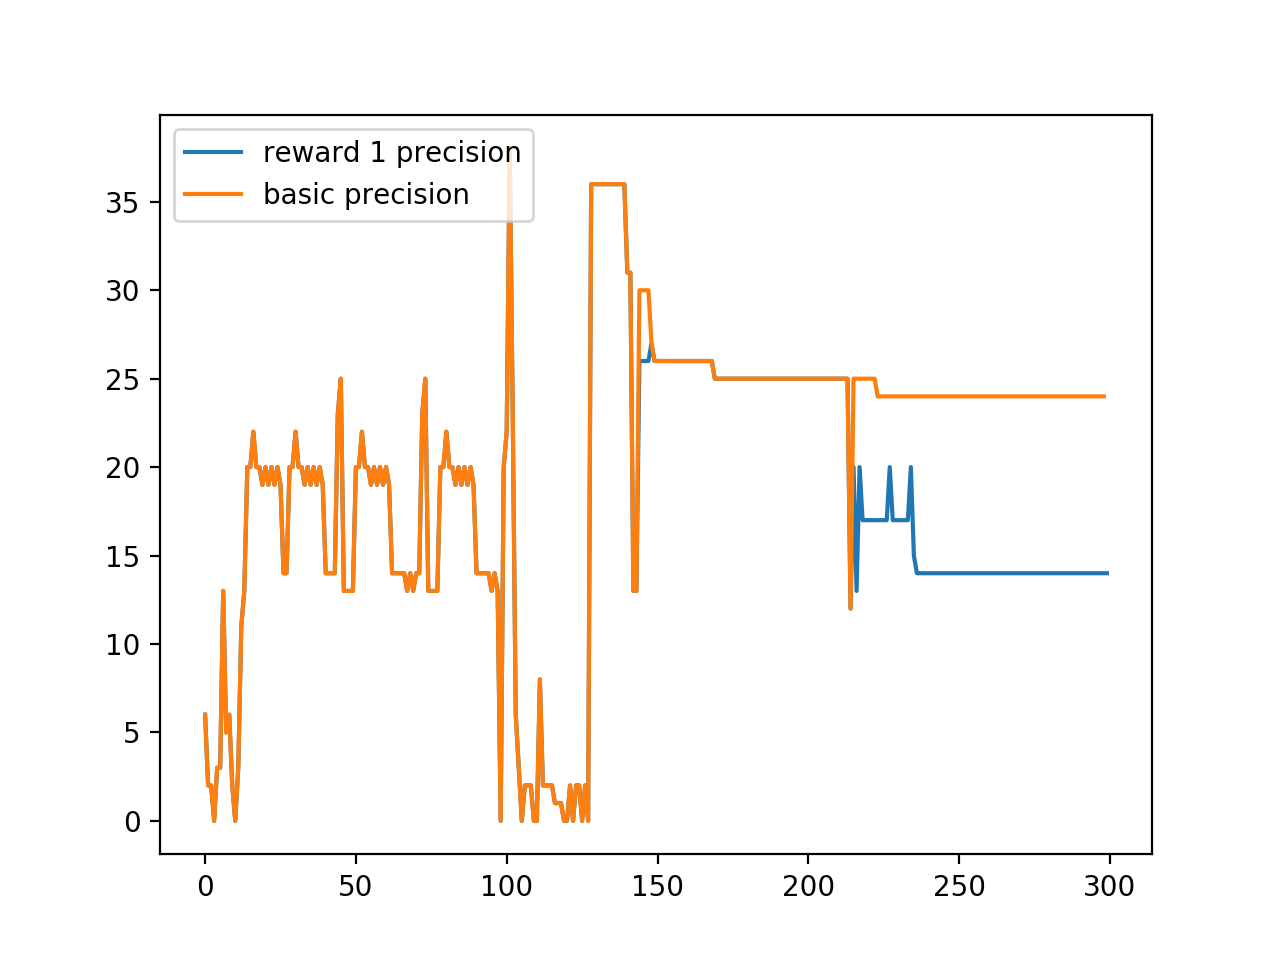
\includegraphics[width=7cm]{figures/r1}
  \caption{Reward one}\label{fig:r1}
\endminipage\hfill
\minipage{0.32\textwidth}
  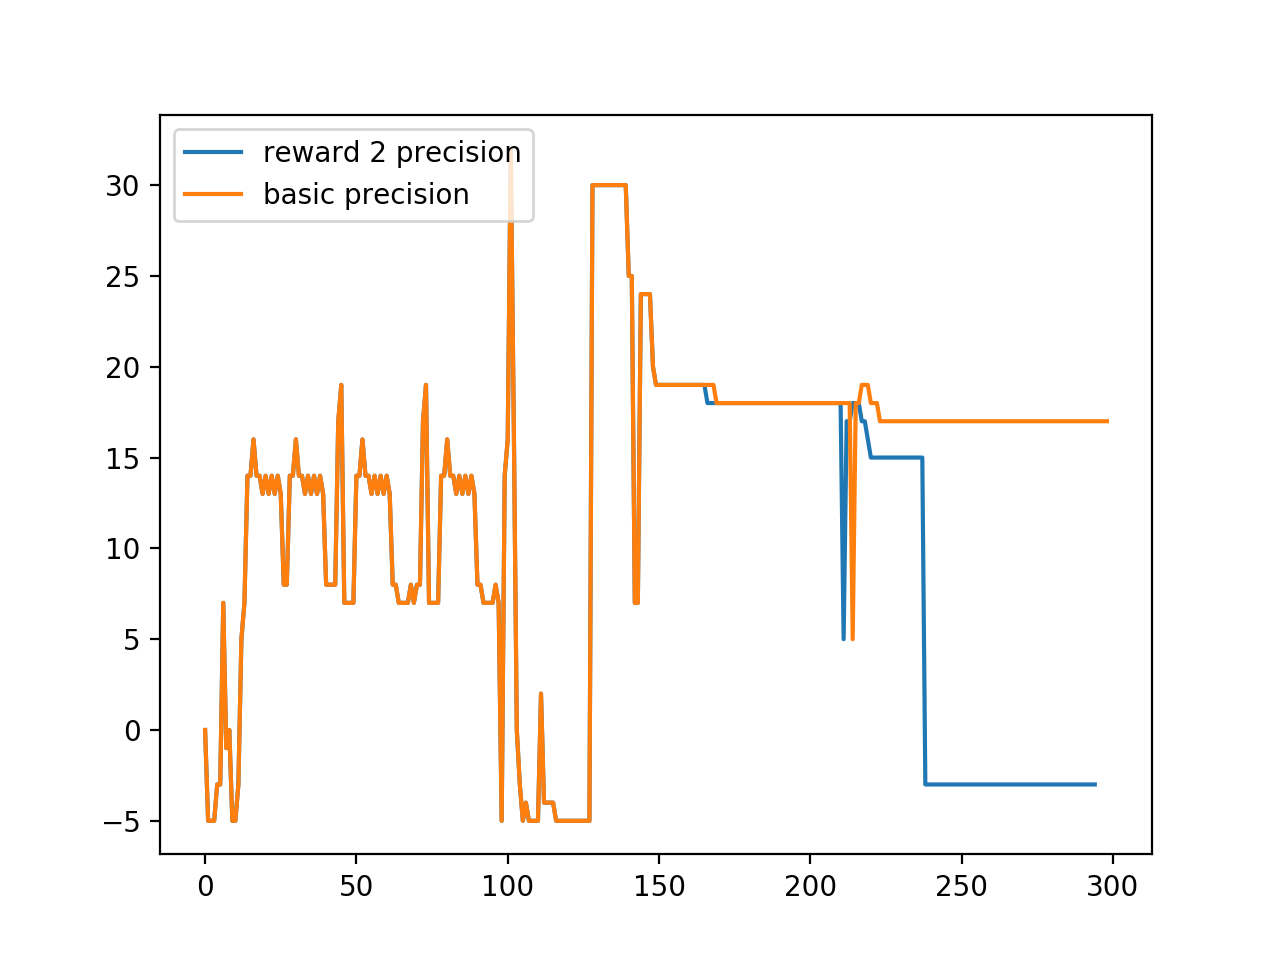
\includegraphics[width=7cm]{figures/r2}
  \caption{Reward two}\label{fig:r2}
\endminipage\hfill
\minipage{0.32\textwidth}%
  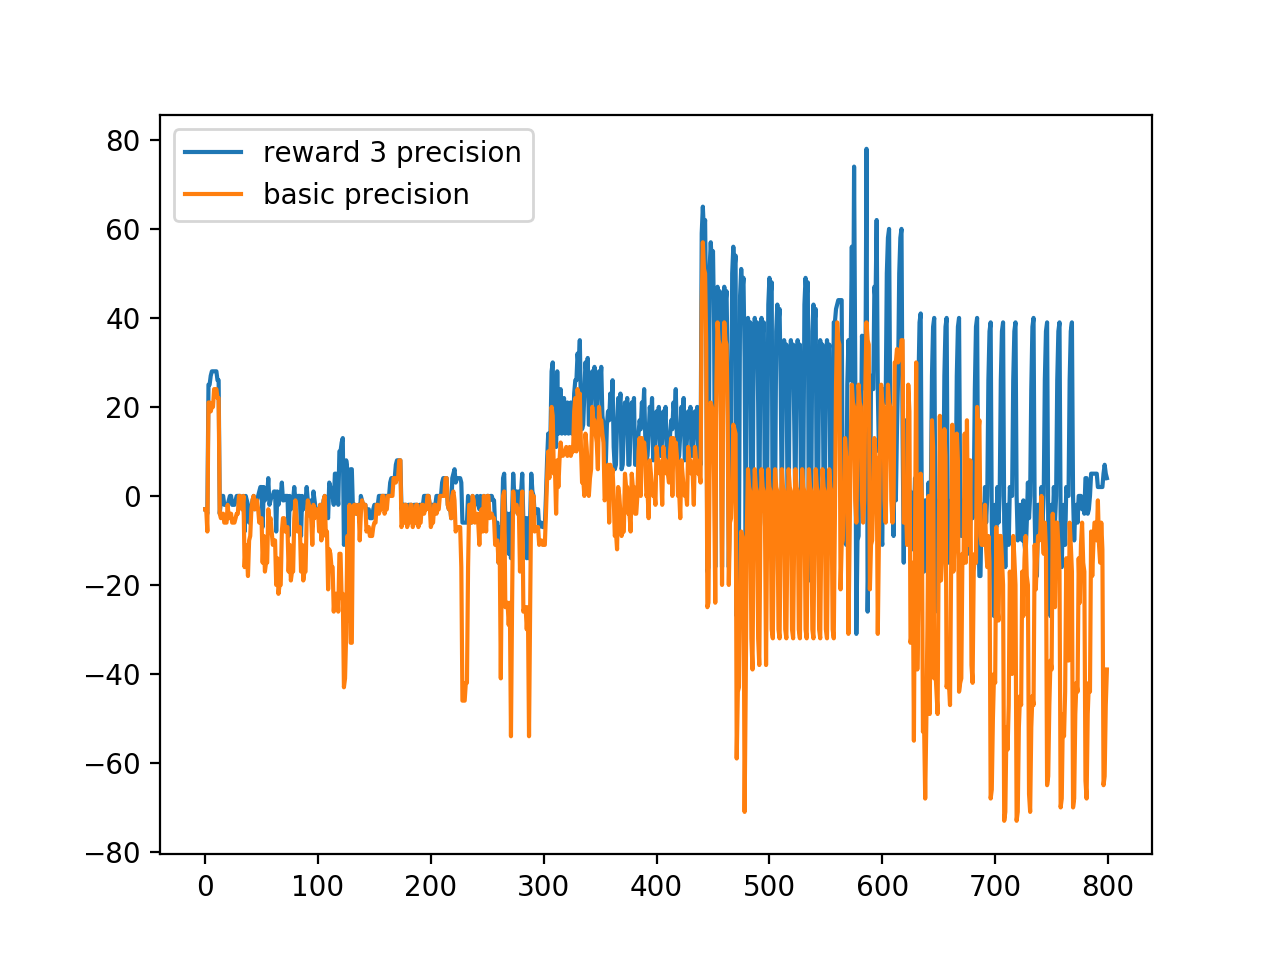
\includegraphics[width=7cm]{figures/r3}
  \caption{Reward three}\label{fig:r3}
\endminipage
\end{figure}

The orange line represents the measured reward whilst running the Q-learning algorithm and the blue line the measured reward of the DQN trained with the corresponding reward. The overall precision of the end polyhedra is the following: For Figure 5.1. 99\% for Q-learning and 96\% for DQN. For figure 5.2. 99\% for Q-learning and 94\% for DQN. For figure 5.3. 97\% for Q-learning and 90\% for DQN. Whilst the graphs behave as expected in the first two scenarios, that is that the reward is lower for the algorithm with lower overall precision as well. In the last graph, we can see something unexpected. Whilst the DQN algorithm has a higher reward throughout most of the execution of the program with an average of 9 versus -8 for the Q-learning algorithm. This indicates that it should also have a better overall precision. However, its overall precision is lower. This tells us that whilst the DQN has learned a correct strategy for maximising the reward, this reward does not guide it to the end goal of maximising the final precision and therefore reward three is not an optimal reward function. These experiments do not give us much information on the differences between reward one and two as they both behave as they should. This is to be expected as reward one and two are similar.\\
It is worth noting that whilst these experiments do give us some interesting information about the effectiveness of the different reward functions, the results are heavily dependant on the benchmark we run them on and therefore the results cannot be fully trusted. However, with the information gathered by these experiments, as well as some overall testing we decided to use the second reward function in further experiments.


\section{Action selection algorithm}
The second problem was selecting the best action selection algorithm. In section 4.3.4., four different action selection algorithms were proposed. In order to select the best one of these, we proceeded by training a DQN using each of them and then comparing the overall precision. Not all the training had to be done separately for the four algorithms. Firstly, we could train estimators from only random actions and then simply specialise each of them with their own action selection algorithm. We then compared the results on a set of seven different benchmarks.
\begin{center}
\captionof{table}{Results of experiments with different action selection algorithms}
\Indm\Indm\Indm\begin{tabular}{||c c c c c c||} 
 
 \hline
 Benchmark & Q-learning & Algorithm 1 & Algorithm 2 & Algorithm 3 & Algorithm 4  \\ [0.5ex] 
 \hline\hline
 driver-media & 99.0 & 98.6 & 97.6 & 93.2 & 98.0 \\ 
 \hline
 linux-kernel-locking-spinlock & 99.9 & 94.4 & 63.6 & 79.9 & 95.0 \\
 \hline
 linux-usb-dev & 58.2 & 51.8 & 60.3 & 56.5 & 59.3\\
 \hline
 linux-kernel-locking-mutex & 77.1 & 73.2 & 95.5 & 95.6 & 76.1\\
 \hline
 complex-emg-drivers-net & 57.1 & 97.3 & 94.6 & 96.0 & 96.9\\ 
 \hline
 complex-emg-drivers-media & 57 & 50.1 & 58.9 & 55.4 & 54.9\\ 
 \hline
 complex-emg-linux-alloc-spinlock & 44.9 & 72.2 & 69.9 & 91.8 & 72.0\\ 
 
 \hline
\end{tabular}
\end{center}

As to the choice of benchmarks for this experiment. We had several criteria. First, we picked benchmarks where achieving a high level of accuracy was not too easy in order to have more informative results. Second, we picked benchmarks that were fast to compute so that the testing time would be fast. We also picked fast benchmarks because the goal was to find an algorithm that maximises the precision as each of these algorithms can be then optimised with their own parameters in order to ameliorate performance and in this way we only had to concentrate on a single goal.\\
As to the results of these experiments. Unfortunately, there is no overall best algorithm. As discussed in section 4.3.4., each of these algorithms has its advantages and shortcomings. However, the main objective we were looking for from these experiments was finding an algorithm that would be stable. We can see that algorithms two and three can obtain very good results on some benchmarks. Unfortunately, their performance is far from optimal on others. This is due to the fact that both of these are strongly threshold dependant and picking an optimal threshold that would work well for all benchmarks is very difficult, making both of these algorithms not practical. Afterwards, between the first and fourth algorithm, the last one outperforms the first on average and therefore is the one we will use from here on. Whilst the last algorithm does not have the best precision on some benchmarks, its stability overall benchmarks made it the preferred candidate.


\section{Final algorithm}
Once both decisions were made, the architecture of the final separated algorithm was fully decided and could, therefore, be further trained and optimised.\\
For the testing of the different algorithms, we decided to run them on a large set of benchmarks. In this way, we could see if they managed to learn a global policy or simply find local minima. In the end, we settled on a set of 81 different benchmarks of varying sizes and complexities. Due to the relatively large number of benchmarks, we set the timeout to be quite short, more specifically thirty minutes. This was done so that the experiments could be run in a reasonable amount of time. For each benchmark, we saved the resulting invariants of the analysis and the runtime.\\
\mbox{}\\
We test the benchmarks using four different analyses:
\begin{itemize}
    \item Using the decomposed Polyhedra domain, to have a baseline for precision.
    \item RL trained with Q-learning
    \item Basic deep Q-network algorithm
    \item Deep Q-network with separated estimators
\end{itemize}

The following table displays the results of the experiments. It shows the average of the precision percentages when compared to the abstraction-less analysis. The total runtime on all benchmarks, the number of benchmarks that the analysis timed out on. The number of benchmarks where the algorithm achieved $100\%$ precision. Finally, for the reinforcement learning algorithms, the number of benchmarks where they outperform the other RL algorithms with regards to precision. 

\begin{center}  
\captionof{table}{Results with final algorithms}
\begin{tabular}{||c c c c c||}
 
 \hline
 Results on 81 bench. & Elina & Q-learning & DQN & Separated DQN \\ [0.5ex] 
 \hline\hline
 Avg. prec. (\%) & 100 & 87.1 & 94.9 & 91.6\\
 Runtime (hr.) & 18:28 & 14:05 & 15:35 & 11:21\\
 $n^{\circ}$ timeouts & 33 & 23 & 23 & 17\\
 $n^{\circ}$ bench. 100\% prec. & 81 & 13 & 27 & 18\\
 $n^{\circ}$ bench. most precise &  & 1 & 36 & 2\\
 
 \hline
\end{tabular}
\end{center}

\subsubsection{Result discussion}
As shown in the results, we were able to outperform the Q-learning method with both the deep Q-network and the separated deep Q-network algorithms with regards to accuracy. What is interesting to note, is that the regular DQN outperforms the separated one in terms of precision. This can most likely be explained by the action selection algorithm. Even though in 5.2., we attempted to pick an algorithm that would be as stable as possible and be able to maintain good results overall benchmarks. The results show that on a few benchmarks the separated DQN performs very poorly, thus reducing its overall precision. However, it is worth noting that the separated DQN outperforms all the other algorithms in terms of performance, as it manages to finish the analysis of all the benchmarks quite a lot faster than the others, most notably, it is faster than the Q-learning algorithm whilst remaining more precise as well. The separated DQN also has the least timeouts out of all the analyses. In terms of precision, however, the normal DQN algorithm is the most precise on average overall benchmarks. It is also more precise on 36 of the 81 benchmarks and is only beaten on one benchmark by Q-learning and on two by the separated DQN, the precision remains the same on the rest. It also achieves $100\%$ precision on more than double the number of benchmarks than the Q-learning method does.  

































% !TEX root = ../thesis.tex

\chapter{Evaluation}

evaluation of the project. user study etc.

\section{Methodology}

general information, in what aspects the system was evaluated

\section{Experiment: Comparison of two Prototypes}

explain idea behind controlled comparison study

\subsection{Setup}

setup of this user experiment

\subsection{Results}

discuss results of the controlled comparison

\section{Experiment: Cognitive Walkthrough}

explain idea behind cognitive walkthrough, what aspects

\subsection{Setup}

setup of the cognitive walkthrough

\subsection{Results}

results of the cognitive walkthrough

\section{Long term study}

explain idea behind long term study, what would be the goal of this experiment

\subsection{Setup}

setup of the long term user study

\subsection{Discussion}

explain issue of time, was not enough to actually perform the study

\section{Limitations}

what are the most significant limitations in the project, how could the be improved in future work
% !TEX root = ../thesis.tex
\chapter{Conclusion}
%TODO continous action space for threshold
In this work, we managed to build a framework for the training and testing of various deep reinforcement learning algorithms inside polyhedra analysis. We could then design a series of such algorithms. These algorithms ranged from very global reinforcement learning methods to ones more optimised with problem-specific knowledge as well as having a greater flexibility towards the various subproblems. We then tested out the different subparts of our algorithms we had come up with, in the goal of finding an optimal combination.\\
Once our algorithms were designed, we could then test them on a broad array of different benchmarks. They outperformed other preexisting reinforcement learning methods on both accuracy and performance.\\
It is also worth noting that we highlighted the overall effectiveness of the global deep Q-network algorithm, as, after all, it was able to craft a decision policy that was the most accurate. Even with the design of new training algorithms that used more domain-specific knowledge, we could only increase the performance at the loss of some precision.\\
Future research for this work could be done in several directions. Techniques such as CNN's could be investigated for automatic feature extraction from the polyhedra itself. Other works such as \cite{dyer1991random, kim2004fast} could also be used for the approximation of the volume of the polyhedra. Both techniques could then be simultaneously used for expanding the features as well as the reward for precision. Other than that, optimisations to the neural network itself could be undertaken as this was not explored much in this work. An expansion of the action set, most notably the size and number of different thresholds, perhaps even using a continuous action set for the size of the threshold could increase the precision. Finally, separating the features, NN's and making them more task-specific, would increase the overall performance.


% ---- END MAIN PART ----


\appendix
\clearpage
\renewcommand*{\chapterpagestyle}{myappendixpagestyle}

% !TEX root = ../thesis.tex

\chapter{Appendix}

in here we put all questionnaires, guides etc.

\section{Controlled Comparison}

questionnaire and guide, script

\subsection{Guides}

guide for controlled comparison

\subsection{Questionnaire}

questionnaires

\section{Cognitive Walkthrough}

questionnaire and guide, script

\subsection{Guides}

guide for cognitive walthrough

\subsection{Questionnaire}

questionnaires

\section{Long Term Study}

questionnaire and guide, script

\subsection{Guides}

guide

\clearpage
\renewcommand*{\chapterpagestyle}{empty}

%\nocite{*}
\cleardoublepage
\phantomsection
\addcontentsline{toc}{chapter}{Bibliography}
\bibliography{bibli}




\end{document}











